
\documentclass[10pt,slovak,a4paper]{article}%twosided

\usepackage[slovak]{babel}
\usepackage[IL2]{fontenc}
\usepackage[utf8]{inputenc}
\usepackage{graphicx}
\usepackage{url}
\usepackage{hyperref} 
\usepackage{cite}
\usepackage[table,xcdraw]{xcolor}
\usepackage[bottom]{footmisc}

\pagestyle{headings}

\title{Využívanie cloudových služieb na zabezpečenie E-learningu v modernom vyučovacom procese\thanks{Semestrálny projekt v predmete Metódy inžinierskej práce, ak. rok 2020/21, vedenie: Mgr. Martin Sabo, PhD.}}

\author{Ján Ágh\\[2pt]
	{\small Slovenská technická univerzita v Bratislave}\\
	{\small Fakulta informatiky a informačných technológií}\\
	{\small \texttt{xagh@stuba.sk}}
	}

\date{\small 19. október 2020}



\begin{document}

\maketitle

\begin{abstract}

Po digitálnej revolúcii si nové technológie, ako napríklad cloudové služby, postupne
našli svoju cestu aj do každodenného vyučovacieho procesu a v dnešnej dobe sa už považujú
za jeho dôležitú súčasť. Ich inklúzia viedla k vzniku množstva nových situácií, ktorým sa
museli prispôsobiť ako učitelia, tak aj žiaci. Medzi najvýznamnejšie z nich bezpochyby patrí
možnosť zdieľania učebných materiálov, ktorá predstavuje primárnu tému článku, a rovnako
fakt, že žiaci a študenti majú prístup k týmto učebným materiálom aj z pohodlia svojho
domova. Cloudové služby taktiež vytvorili základ pre vznik „virtuálnych tried“, pomocou
ktorých učitelia a študenti dokážu komunikovať aj bez potreby osobného stretnutia sa.
Nemenej dôležité sú aj skutočnosti, že cloudové služby vnášajú chýbajúcu flexibilitu do
vyučovania a podporujú znižovanie nákladov v oblasti informačných systémov.
\end{abstract}



\section{Úvod do problematiky}

Navštevovanie školy a zúčastňovanie sa vyučovacieho procesu je dlhodobo integrálnou súčasťou života každého mladého človeka. Už v počiatkoch ľudskej civilizácie bol kladený veľký dôraz na poskytnutie čo najobsiahlejšieho vzdelania mladším príslušníkom spoločnosti, pretože práve títo jedinci sú kľúčoví pri budúcom rozvoji ľudského poznania. Ani dnes tomu nie je inak. Napriek tomu môžeme vidieť, že tradičná prezenčná výučba, akú poznáme niekoľko storočí, je veľmi krehká a isté skutočnosti, ako napríklad pandémia COVID-19, ju dokážu reálne ohroziť, v niektorých prípadoch dokonca prerušiť. Riešenie na tento problém predstavuje neustála modernizácia už zastaralých postupov, ktorá v dnešnej modernej dobe bezpochyby zahrňuje aj postupnú integráciu cloudových služieb do vyučovania\cite{Koutsopoulos_schooloncloud}. Tieto služby dokážu zjednodušiť mnoho aspektov vyučovania a v krajných situáciách umožňujú presun celého vyučovacieho procesu do online prostredia. 



\section{Vysvetlenie základných pojmov}


V článku sa často používajú slovné spojenia, ako napríklad cloudové služby alebo E-Learning, ktorým je dôležité porozumieť pred pokračovaním v čítaní.


\subsection{Definícia cloudových služieb}


Cloudové služby by sme vedeli definovať ako súhrnné pomenovanie rôznych aplikácií, úložného priestoru, počítačových sietí a sieťových služieb, ktoré sú umiestnené na určitom serveri, prípadne na Internete, pričom hlavnou požiadavkou je to, aby mali používatelia prístup k týmto službám z viacerých lokalít, t.j. z domáceho prostredia, pracovného prostredia a podobne\cite{Babu_enrichingeducation}\cite{Narkar_cloud-basededucation}. Na druhej strane, predpokladom na pripojenie sa k daným službám je vlastníctvo výpočtových zariadení, ako osobné počítače a mobilné telefóny, a vo väčšine prípadov aj prístup k Internetovému pripojeniu. Dôležitou vlastnosťou cloudových služieb je aj to, že vyžadujú iba minimálnu úroveň údržby a správy zo strany poskytovateľa služieb, pričom používateľom ponúkajú vysokú úroveň zabezpečenia\cite{Babu_enrichingeducation}.  

\subsection{Definícia pojmu E-learning}


Mhouti, Erradi a Nasseh definujú pojem E-Learning nasledovným spôsobom: \uv{E-Learning je oblasť súvisiaca s virtualizovanou online výučbou s využitím synchrónnych a asynchrónnych komunikačných mechanizmov, konkrétne Internetu\cite{Mhouti_benefits_challenges}.} E-Learning umožňuje pedagógom udržiavať kontakt so svojimi študentmi aj v prípadoch, kedy sa z rozličných dôvodov nemôžu zúčastniť vyučovacieho procesu osobne. Počas E-Learningu sa vo veľkej miere využívajú služby poskytované cloudom, konkrétnejšie úložný priestor na zdieľanie učebných materiálov a aplikácie, cez ktoré dokážu pedagógovia a študenti komunikovať v reálnom čase.  

\section{Potreba integrácie cloudu do vyučovania}


Existuje viacero objektívnych dôvodov, prečo je dôležité integrovať služby ponúkané cloudom a iné moderné technológie do každodenného vyučovacieho procesu. Medzi najdôležitejšie dôvody jednoznačne patrí to, aby študenti boli s týmito technológiami oboznámení a vedeli ich správne používať, pretože mnoho kvalitných pracovných pozícií v dnešnej dobe vyžaduje vysokú znalosť týchto technológií\cite{Babu_enrichingeducation}. Nemenej dôležitá je aj modernizácia učebného materiálu a jeho dopĺňanie o nové relevantné poznatky, pretože veľká časť školského učiva, ktoré sa dnešní študenti musia naučiť, je zastaralá a preto informácie v nich obsiahnuté študenti nedokážu vo svojom ďalšom zameraní využiť.
\\
\\
Na druhej strane, pre školy a iné vzdelávacie inštitúcie je kľúčové znižovanie svojich výdavkov bez toho, aby tým bola zasiahnutá kvalita poskytovaného vyučovania. Namiesto implementácie vlastných komplexných hardvérových a softvérových systémov sa tak môžu tieto inštitúcie prikloniť k používaniu systémov a aplikácií uložených na cloude, ktoré poskytujú v princípe rovnaké služby, ale za výrazne nižšie poplatky\cite{Mhouti_benefits_challenges}. Za zmienku stojí aj fakt, že školy nie sú zodpovedné za údržbu alebo aktualizáciu týchto cloudových systémov a aplikácií, nakoľko oni nie sú vlastníkmi, čím vzniká priestor na ďalšie znižovanie výdavkov\cite{Narkar_cloud-basededucation}.


\section{Využitie cloudu vo vyučovaní}

Cloudové služby predstavujú priamočiary spôsob, ktorým je možné zjednodušiť, urýchliť a zmodernizovať väčšinu oblastí vyučovacieho procesu. V diagrame nižšie sú vymenované niektoré z týchto oblastí.

\begin{figure}[h]
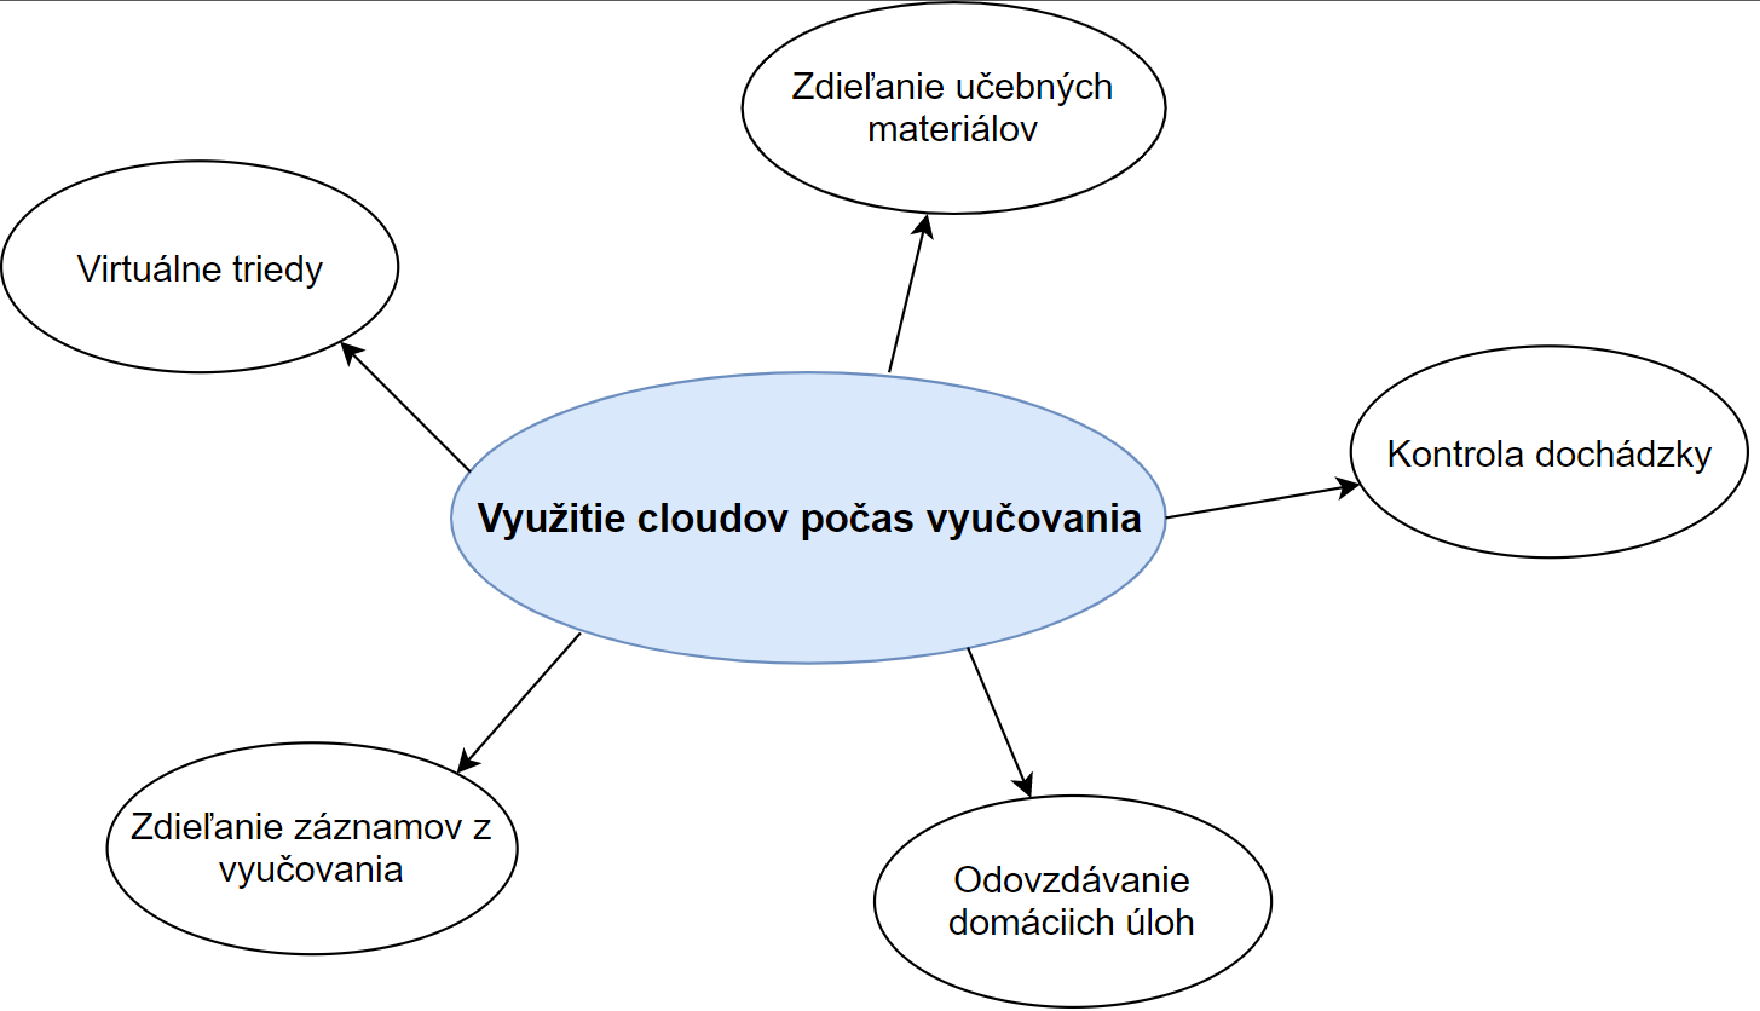
\includegraphics[width=1\textwidth]{Obrázky/cloud_diagram.pdf}
\caption{Viacero spôsobov využitia cloudov vo vyučovaní.}
\end{figure}

Najčastejšie spomínanou oblasťou je bezpochyby zdieľanie učebných materiálov a domácich úloh. Na tento účel sa obvykle používajú cloudové úložné priestory dostupné online. Ich hlavnou výhodou je fakt, že si žiaci a učitelia môžu prezerať a meniť zdieľaný obsah z akejkoľvek lokality vybavenej internetovým pripojením. Aplikácie využívajúce cloudové služby sa v dnešnej dobe taktiež začínajú úspešne presadzovať v oblasti zaznamenávania dochádzky žiakov a zapisovania známok. Ponúkajú oveľa vyššiu flexibilitu v porovnaní k papierovým triednym knihám a v prípade zadania nesprávneho údaju je ho možné okamžite upraviť, čo by pri papierových triednych knihách bolo problematické. Okrem vyššie uvedených oblastí sa, hlavne kvôli súčasnej pandemickej situácii, stali zástupcami tradičnej prezenčnej výučby a mnoho škôl ich využíva na poskytovanie vyučovania pomocou virtuálnych tried a tiež zdieľanie záznamov z vyučovania.


\section{Architektúra cloudových služieb}


Zjednodušená architektúra typického systému kombinujúceho cloudové služby a koncept e-learningu vo väčšine prípadov pozostáva z troch hlavných vrstiev. Prvou a z pohľadu používateľa najdôležitejšou vrstvou je vrstva spájajúca používateľské rozhranie so samotnými cloudovými službami\cite{Mhouti_benefits_challenges}. Táto vrstva umožňuje používateľovi interakciu s cloudom, t.j. nahrávanie a sťahovanie obsahu z cloudových úložísk a jeho hlavnou požiadavkou je jednoduchosť a priamočiarosť dizajnu, aby používateľ mohol využívať systém bez väčších ťažkostí. Nasledujúca, druhá vrstva je zodpovedná za zabezpečenie cloudových služieb rôznych typov, ako napríklad IaaS (Infrastructure as a service) pre cloudové úložné priestory, Saas (Software as a service) pre mailové služby a prácu s rôznymi protokolmi a PaaS (Platform as a service) umožňujúci vývoj vlastných systémov, pričom dôležitou vlastnosťou je to, že sa používateľ nemusí zaoberať údržbou a aktualizáciou týchto služieb, nakoľko on nie je ich vlastníkom\cite{Mhouti_benefits_challenges}. Posledná, tretia vrstva reprezentuje kompletnú hardvérovú výbavu systému, ako napríklad pamäte, procesory alebo iné aktívne aj pasívne prvky, a ich údržbu\cite{Mhouti_benefits_challenges}.


\section{Výhody a problémy spojené s využívaním cloudu}

\subsection{Výhody cloudových služieb}


Z využívania cloudových služieb na zjednodušenie viacerých aspektov vyučovacieho procesu plynie mnoho významných výhod ako pre študentov, tak aj pre rôzne vzdelávacie inštitúcie, ktoré títo študenti navštevujú. Tieto služby dokážu v kombinácii s procesom E-learningu zvýšiť produktivitu pedagógov a študentov tým, že im ponúkajú viacero spôsobov interakcie a uľahčujú túto interakciu medzi nimi, a taktiež podporujú spoluprácu medzi študentmi ako jednotlivcami\cite{Mhouti_benefits_challenges}. Nemenej dôležitý je aj fakt, že žiaci a učitelia nepotrebujú žiadne špeciálne školenie na to, aby dokázali tieto systémy správne používať a k zdieľaným materiálom majú prístup prakticky z akéhokoľvek miesta vybaveného internetovým pripojením\cite{Koutsopoulos_schooloncloud}. Medzi pozitíva patrí aj to, že zásluhou týchto systémov môže každodenné vyučovanie neprerušene prebiehať aj v prípadoch, kedy realizácia tradičného prezenčného vyučovania nie je možná, a v neposlednom rade modernizácia jednej časti vyučovacieho procesu postupom času vynúti aj modernizáciu iných častí.
\\
\\
Pre vzdelávacie inštitúcie môže byť zaujímavá hlavne nízka cena implementácie takéhoto systému a tiež prakticky nulové poplatky za údržbu a aktualizáciu súčastí systému\cite{Narkar_cloud-basededucation}. Ďalšie veľké výhody predstavujú obrovský úložný priestor dostupný online za veľmi nízke poplatky a vysoká úroveň zabezpečenia proti odcudzeniu dát a údajov uložených na danom cloude\cite{Mhouti_benefits_challenges}. 
\\
\\
Cloudové služby pri pohľade na budúcnosť prinášajú výhody aj pre svojich vlastníkov. Rozmachu cloudových služieb vo veľkej miere pomohla súčasná pandemická situácia, kedy bolo školstvo v celom svete doslova prinútené ich začať používať. Oblasť cloudových služieb sa tak zrazu stala veľmi zaujímavou z ekonomického hľadiska a mnoho veľkých spoločností sa rozhodlo do nej preinvestovať veľkú časť svojich zdrojov s cieľom využiť situáciu a dosiahnuť čo najväčšie zisky. Pre princíp ilustrácie sú v tabuľke nižšie zobrazené zisky spoločnosti Zoom Video Communications od jej založenia, pričom obrovský nárast ziskov počas pandémie je zvýraznený farebne.

\begin{table}[h]
\centering
\begin{tabular}{|l|c|c|c|c|}
\hline
              & \multicolumn{1}{l|}{\textbf{1. kvartál}} & \multicolumn{1}{l|}{\textbf{2. kvartál}} & \multicolumn{1}{l|}{\textbf{3. kvartál}} & \multicolumn{1}{l|}{\textbf{4. kvartál}} \\ \hline
\textbf{2018} & 0\$                                      & 60 mil. \$                               & 75 mil. \$                               & 90 mil. \$                               \\ \hline
\textbf{2019} & 106 mil. \$                              & 122 mil. \$                              & 146 mil. \$                              & 167 mil. \$                              \\ \hline
\textbf{2020} & \cellcolor[HTML]{FFCCC9}188 mil. \$      & \cellcolor[HTML]{FFCCC9}328 mil. \$      & \cellcolor[HTML]{FFCCC9}664 mil. \$      & N/A                                      \\ \hline
\end{tabular}
\caption{Zisky Zoom Video Communications od jej založenia.}
\end{table}


\subsection{Problémy s cloudovými službami}

Samozrejme, ako to s každou modernizáciou chodí, aj pri integrácii cloudu do vyučovacieho procesu sa môžu objaviť isté problémy. Tieto problémy najčastejšie spôsobujú príslušníci staršej generácie, ktorí sú prispôsobení svojim zažívaným praktikám vrámci prezenčného vyučovania a iba neradi by sa adaptovali novým technológiám. Významné problémy môžu byť vyvolané aj nevyhovujúcou finančnou situáciou škôl, kedy jednoducho nemajú peňažné prostriedky na modernizáciu. Na záver, ale v neposlednom rade závisí modernizácia v oblasti školstva a všeobecne inklúzia cloudových služieb aj od finančného stavu krajiny, v ktorej sa nachádzajú. Študenti pochádzajúci z menej majetných krajín tak majú automaticky istú nevýhodu v porovnaní k študentom z bohatších krajín, kde modernizácia školstva prebieha rýchlejšie.
%Okrem toho modernizácia vyučovania zapríčiňuje rozsiahle zmeny aj v postavení a úlohách pedagógov a študentov\cite{Koutsopoulos_schooloncloud}. Hlavnou úlohou pedagógov naďalej ostáva umožniť študentom nadobudnúť potrebné poznatky a vzdelanie, ale kým doteraz bolo ich poslaním prezentovanie nových poznatkov na vyučovacích hodinách, odteraz sa od nich očakáva prevažne aktívnejší prístup, ktorého cieľom je uľahčiť študentom vzdelávanie\cite{Koutsopoulos_schooloncloud}. Dôvod je to, že učitelia už nie sú jediným dostupným zdrojom informácií pre študentov. V tejto oblasti boli z veľkej časti nahradení online databázami a službami, ktoré študentom ponúkajú rýchlejší prístup k požadovaným informáciám.%


\section{Záver}

Dovôdy a argumenty spomenuté v tomto článku jasne ukazujú, že budúcnosť vyučovacieho procesu je úzko spätá s vývojom cloudových služieb a aplikácií. Využívanie cloudových služieb prináša výhody obom stranám - študenti si osvoja prácu s nimi a nadobudnú dôležité skúsenosti, ktoré budú môcť zúžitkovať vo svojom budúcom povolaní, a školské a iné vzdelávacie inštitúcie môžu dramaticky zvýšiť kvalitu poskytovaného vyučovania a medzitým ešte aj ušetriť, pričom majú priestor spotrebovať ušetrené peňažné prostriedky na ďalšiu modernizáciu vyučovania.

%\begin{figure}
%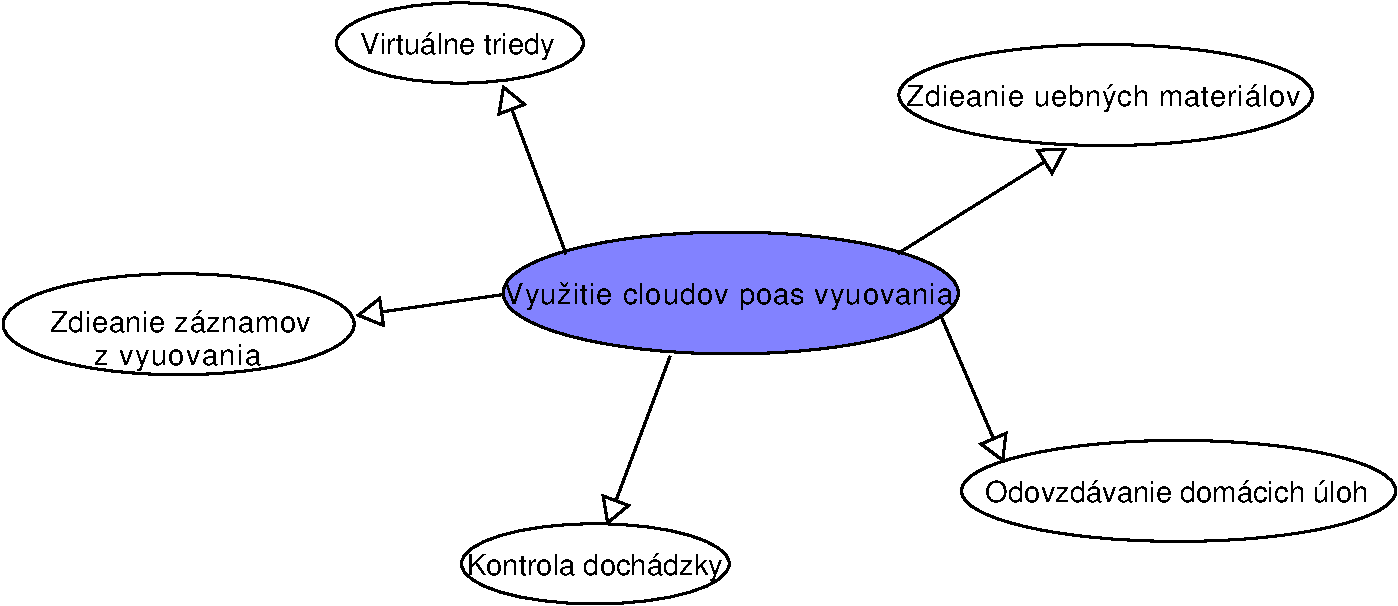
\includegraphics[width=1\textwidth]{Obrázky/opis-crop.pdf}
%\caption{Prvý diagram}
%\end{figure}


\bibliography{literatura}
\bibliographystyle{unsrt}
\end{document}
